% Compile with XeLaTeX or Tectonic. Portrait: ../site/public/profile.jpg.
\documentclass[10pt,a4paper]{article}
\usepackage[a4paper,left=12mm,right=12mm,top=10mm,bottom=13mm]{geometry}
\usepackage{fontspec}
\setmainfont{lmroman10-regular.otf}[BoldFont=lmroman10-bold.otf,ItalicFont=lmroman10-italic.otf,BoldItalicFont=lmroman10-bolditalic.otf]
\usepackage{graphicx}
\usepackage{enumitem}
\usepackage{titlesec}
\usepackage{hyperref}
\hypersetup{hidelinks,pdftitle={CV - Ung Nhut Khang - Web Developer},pdfauthor={Ưng Nhựt Khang}}
\pagestyle{empty}
\setlength{\parindent}{0pt}
\setlength{\parskip}{0pt}
\setlist[itemize]{leftmargin=12pt,itemsep=1pt,topsep=2pt,parsep=0pt}
\titleformat{\section}{\fontsize{12.5}{15}\selectfont\bfseries}{}{0pt}{}[\vspace{1pt}\titlerule]
\titlespacing*{\section}{0pt}{7pt}{4pt}
\newcommand{\project}[2]{\textbf{#1}\hfill #2\par}
\newcommand{\projectmeta}[2]{{\fontsize{9}{11}\selectfont\itshape #1\hfill #2}\par}
\begin{document}
\fontsize{10}{12}\selectfont

\begin{minipage}[c]{28mm}
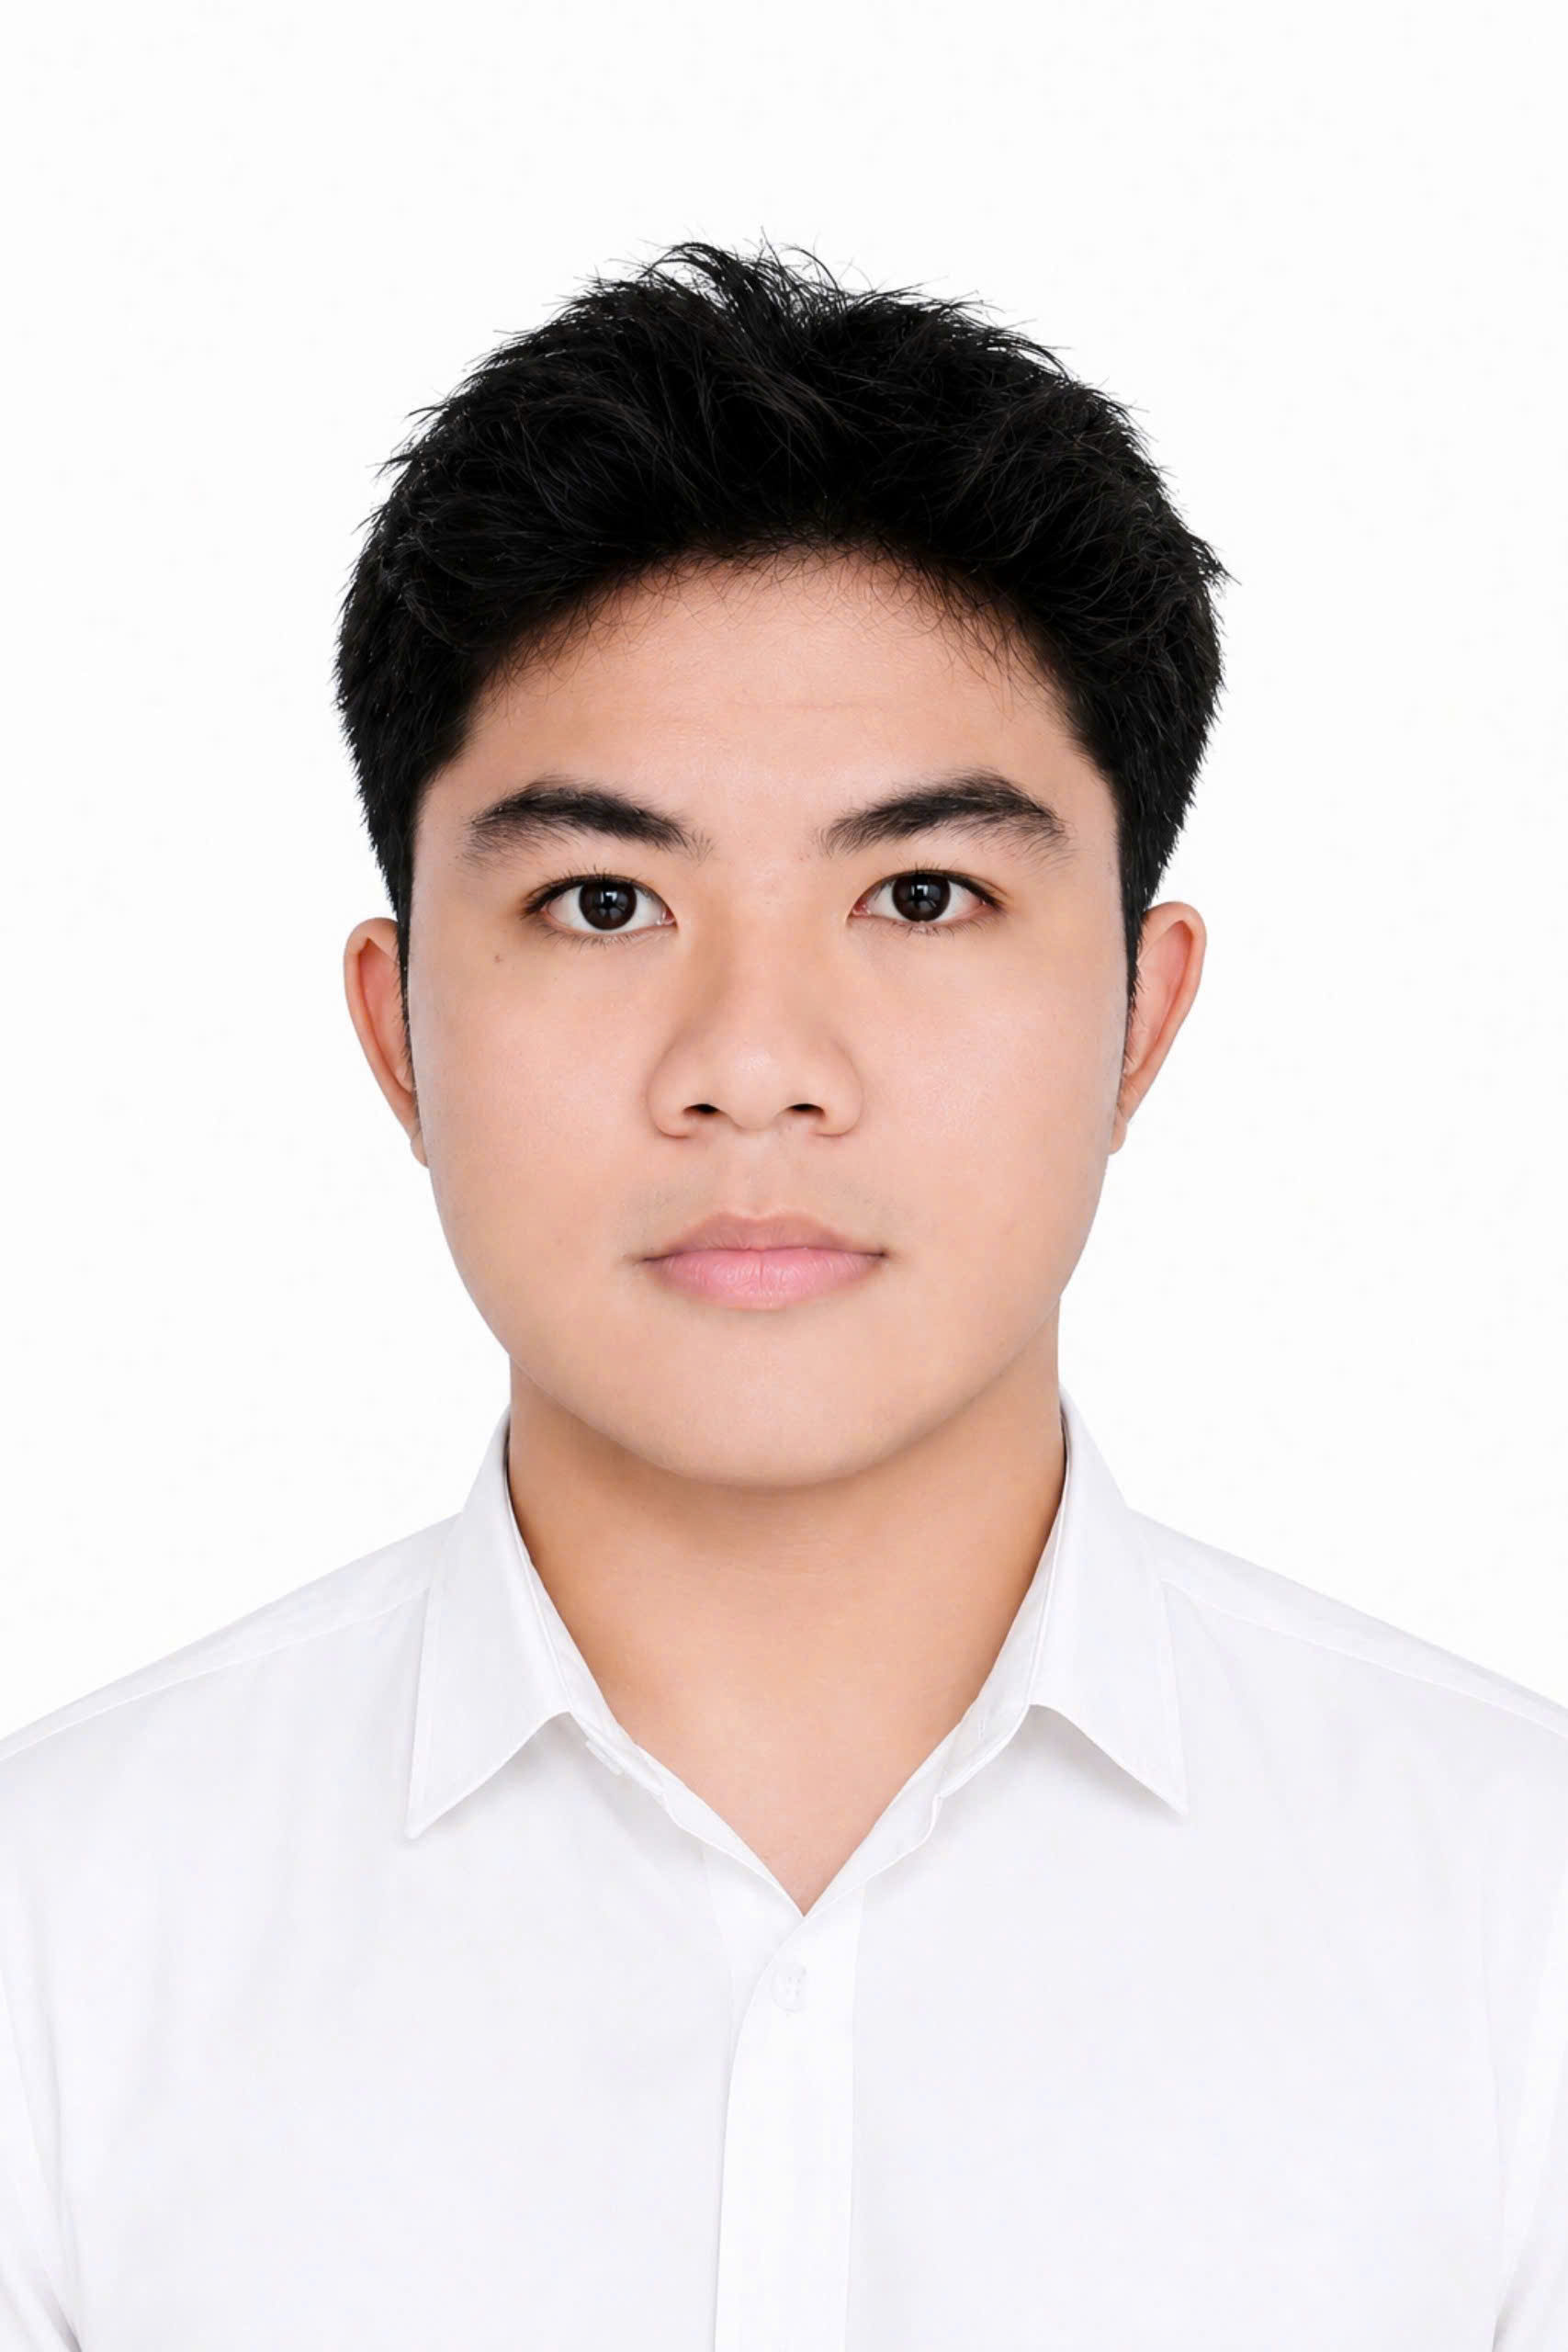
\includegraphics[width=28mm]{../site/public/profile.jpg}
\end{minipage}\hspace{4mm}%
\begin{minipage}[c]{153mm}
{\fontsize{19}{23}\selectfont\bfseries ƯNG NHỰT KHANG}\par
\vspace{3pt}
{\fontsize{10.5}{13}\selectfont\bfseries Web Developer}\par
\vspace{3pt}
Information Technology student, majoring in Software Engineering\par
\vspace{5pt}
\textbf{Email:} \href{mailto:contact@ungnhutkhang.id.vn}{contact@ungnhutkhang.id.vn}\hspace{5mm}\textbf{Phone:} 0393 331 566\par
\vspace{2pt}
\textbf{Location:} Cat Lai Ward, Ho Chi Minh City, Vietnam\par
\vspace{2pt}
\textbf{GitHub:} \href{https://github.com/mm4you}{github.com/mm4you}\par
\vspace{2pt}
\textbf{Website:} \href{https://www.ungnhutkhang.id.vn/}{ungnhutkhang.id.vn}
\end{minipage}
\vspace{5pt}
\hrule height 0.4pt
\vspace{5pt}

\section{Career objective}
Software Engineering student at UMT seeking a web development internship. Hands-on experience with React, Next.js, TypeScript, databases and API integration through personal and team projects. An independent learner who uses AI tools to support coding and is eager to contribute to real projects.

\section{Education}
\textbf{Ho Chi Minh City University of Management and Technology (UMT)}\hfill 2024 - present\par
\textit{Information Technology, majoring in Software Engineering (SE)}
\begin{itemize}
\item Current GPA: \textbf{3.31}. Expected graduation: \textbf{2028}.
\end{itemize}

\section{Projects}
\project{IELTS Vocabulary}{\href{https://ielts.ungnhutkhang.id.vn/}{Live} / \href{https://github.com/mm4you/ielts}{GitHub}}
\projectmeta{Personal project / IELTS vocabulary app}{Next.js, TypeScript, Tailwind CSS, Prisma, PostgreSQL}
\begin{itemize}
\item SM-2 spaced repetition, practice games and pronunciation; sign-in, saved learning data and progress tracking.
\end{itemize}
\vspace{2pt}
\project{InnovateX Smart Port}{2025 / \href{https://github.com/mm4you/hackathon}{GitHub}}
\projectmeta{Sole developer / Team-developed concept}{Next.js, TypeScript, Prisma, PostgreSQL}
\begin{itemize}
\item Port scheduling, appointment management, operations dashboards and green credits. \textbf{Top 20 (Semifinalist)}, Digiport Logistics Hackathon 2025.
\end{itemize}
\vspace{2pt}
\project{Vô Tri}{\href{https://votrihub.vercel.app/}{Live} / \href{https://github.com/mm4you/votri}{GitHub}}
\projectmeta{Personal project / Browser games}{JavaScript, Three.js, Web Audio API, HTML, CSS}
\begin{itemize}
\item Splash Swim and Wobbly Bird with 3D scenes, physics and audio; Vietnamese/English support, settings and records saved in the browser.
\end{itemize}
\vspace{2pt}
\project{Thi Tho - Live Quiz Gameshow}{\href{https://thitho.vercel.app/}{Live} / \href{https://github.com/mm4you/thitho}{GitHub}}
\projectmeta{Personal project / Realtime quiz gameshow}{Next.js, TypeScript, Supabase Realtime, Tailwind CSS}
\begin{itemize}
\item A four-player quiz system with an MC/judge control panel and stage display; synchronized answers, countdowns and scores, with buzzer and scoring controls.
\end{itemize}
\vspace{2pt}
\project{Drive Music}{\href{https://github.com/mm4you/drive-music}{GitHub}}
\projectmeta{Personal project / Web music player}{React, Next.js, Media Session API, PWA}
\begin{itemize}
\item FLAC playback, playlists and lock-screen controls; a responsive interface with installable PWA support.
\end{itemize}
\vspace{2pt}
\project{CSVC UMT (Facilities Management)}{\textit{In development}}
\begin{itemize}
\item A team web application for facilities management at UMT. Role: Development team member.
\end{itemize}

\section{Technical skills}
\begin{tabular}{@{}p{37mm}@{\hspace{3mm}}p{146mm}@{}}
\textbf{Frontend:} & JavaScript, TypeScript, React, Next.js, Tailwind CSS, Responsive UI.\\[3pt]
\textbf{Backend:} & Next.js API Routes, RESTful API, Prisma ORM, basic authentication.\\[3pt]
\textbf{Databases:} & PostgreSQL, MySQL, Supabase.\\[3pt]
\textbf{Tools:} & Git, GitHub, Vercel.\\[3pt]
\textbf{AI-assisted coding:} & Adapt to AI tools for documentation research, coding assistance and debugging.\\[3pt]
\textbf{English:} & B1-B2 (self-assessed, not certified).
\end{tabular}

\section{Interests}
Meeting friends, conversations over coffee, music and films.
\end{document}
